\chapter{Guida Admin}
\label{app:admin}

\begin{wrapfigure}{r}{0.32\textwidth}
  \begin{center}
    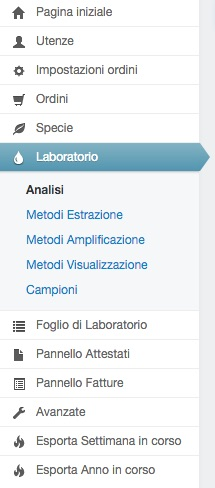
\includegraphics[width=0.3\textwidth]{images/suit}
  \end{center}
\end{wrapfigure}

Il pannello admin Django del Portale Avifauna deve permettere di controllare ogni passo del sistema.

\section*{Utenze}
Un \textsf{utente} del sistema é un entità identificata da un univoco indirizzo email, con password e nominativo. Esso ha attributi booleani per indicare se é attivo, se ha privilegi di staff o da superutente; é inoltre possibile indicare i singoli privilegi in un apposito elenco.

Un \textsf{cliente} invece é un entità associata ad un utente, con tutti gli attributi personali come nome, cognome, codice fiscale/partita iva, indirizzo, contatti telefonici e attributi di sistema come lo schema prezzi associato, la lingua oreferita, la quantità di crediti FEM in possesso e l'eventuale collegamento ad una associazione.

Le \textsf{associazioni} sono caratterizzate da un nome univoco, uno schema prezzi associato e eventuali informazioni aggiuntive.

Per indicare la correlazione tra cliente ed associazione esiste l'entità \textsf{iscrizione ad associazione} con il nominativo del cliente, l'associazione collegata e il numero di tessera corrispondente.

É stato inoltre aggiunto l'attributo booleano \texttt{ufficiale} per permettere agli addetti di {\fem} di indicare quando l'iscrizione del cliente all'associazione corrisponde al vero, poiché il registro degli iscritti di ogni associazione é aggiornato continuamente ma inviato a {\fem} solo ad intervalli temporali.

\section*{Impostazioni ordini}
In questa sezione si trovano quelle opzioni impostabili una tantum che non subiscono frequenti variazioni o controlli.

Vengono raccolti gli \textsf{schemi di prezzi} creati, indicati dal nome e contenenti le tariffe di ogni analisi e attestato; hanno la possibilità di essere di due tipi: Convenzioni o Pacchetti. 

Nel primo caso (tipico di associazioni o clienti professionisti che analizzano un range di specie ridotto) vengono impostati i costi delle analisi come convenzionati, l'ulteriore costo scontato in caso di superamento di una soglia minima dell'ordine e la soglia da superare; vengono anche elencate le specie sulle quali effettuare i prezzi favorevoli e quali invece mantengono il prezzo di listino.

Nel secondo caso invece vanno impostati anche i prezzi scontati di tutte le analisi da applicare in caso di combinazione tra più analisi richieste sullo stesso soggetto.

Vengono anche indicate le cifre dei \textsf{pacchetti crediti FEM} acquistabili, ovvero il prezzo di ciascuno e il credito che il cliente accumula.

Infine si possono impostare e modificare i \textsf{template messaggi}, cioè i messaggi pre-popolati che possono essere utilizzati nelle fasi di invio comunicazioni automatiche. Ogni template ha un nome identificativo univoco, descrizione e ordinamento opzionali e i corpi del testo divisi per ogni lingua.

\section*{Ordini}
Gli \textsf{ordini} sono descritti da campi non modificabili manualmente come il suo stato, l'ammontare e il cliente associato; contengono note fiscali o interne e mostrano la lista di campioni associati con la possibilità di indicare eventuali problematiche di ogni singolo campione. Viene fornita la possibilità di assegnare un \texttt{idLab} (numero sequenziale per il laboratorio) ad ogni campione in modo da procedere con le analisi. 

É anche possibile comunicare direttamente con il cliente attraverso l'apposito tasto \texttt{Messaggi} che apre un editor WYSIWYG (acronimo dall'inglese What You See Is What You Get) ovvero un editor testuale per la scrittura istantanea ed immediata di un messaggio diretto al cliente.

La sezione \textsf{campioni} permette una vista completa di tutti i campioni richiesti da analizzare in una tabella in cui viene indicato il numero dell'ordine di ciascun campione, l'identificativo e la specie. É possibile inoltre modificare alcune informazioni del campione per andare incontro ad eventuali errori di battitura.

In \textsf{acquisto crediti} é possibile visualizzare tutte le transazioni relative all'acquisto di pacchetti crediti FEM ed eventualmente effettuare modifiche.

\section*{Specie}
La possibilità di aggiornare la lista di \textsf{specie} e \textsf{sottospecie} é essenziale per il continuo aggiornamento e sviluppo del lavoro di analisi da parte di {\fem}; per renderlo possibile in una sezione apposta del pannello admin viene presentato l'elenco di specie e sottospecie presenti, con la possibilità di aggiornare, modificare e completare le relative informazioni, tra cui i nomi comuni e le immagini.

\section*{Laboratorio}
La sezione dedicata al laboratorio é uno dei punti cruciali in cui viene svolto la maggior parte del lavoro da parte dei tecnici di {\fem}; é quindi necessario elencare tutte le analisi da eseguire riferite ai relativi campioni, aggiungendo informazioni specifiche come i metodi di estrazione ed amplificazione del DNA in funzione all'analisi richiesta. 

Essendo un ambito ancora in fase di ricerca non é detto che una metodologia scelta corrisponda per forza alla migliore, per questo motivo sono state create le sezioni \textsf{metodo estrazione}, \textsf{metodo amplificazione}, \textsf{metodo visualizzazione} per effettuare i dovuti aggiornamenti. Sono stati inoltre inseriti tre campi di tipo \tag{select} in ogni analisi per permettere ai tecnici di cambiare la metodologia scelta in caso di nuove sperimentazioni. É stato creato per questo il meccanismo del 'processamento multilplo' che permette di effetturare piu volte la stessa analisi su un campione, archiviando i dati relativi a ciascun processamento.

É importante questa struttura per la creazione del \textsf{foglio di laboratorio}.

\section*{Foglio di laboratorio}
Il \textsf{foglio di laboratorio} é una tabella dinamica creata e popolata in una sezione apposta del pannello admin che viene popolata con le analisi da effettuare (cioè che non hanno un esito finale già stabilito).

Questa tabella oltre ad indicare informazioni classiche come l'identificativo del campione, il numero dell'ordine di riferimento e il numero progressivo di laboratorio (idLab), indica di preciso la specie e le analisi da effettuare, lasciando uno spazio per le note da inserire durante il processamento e le metodologie consigliate. Essa viene stampata dal tecnico attraverso l'apposito tasto che genera un pdf e tramite codice {\js} apre una finestra di dialogo diretta per la stampa.

\section*{Pannello attestati e Pannello fatture}
I pannelli di attestati e fatture sono tabelle analoghe al foglio di laboratorio che però servono nelle fasi finali del flusso di ogni ordine.

Il \textsf{pannello attestati} elenca gli ordini che richiedono una stampa cartacea degli attestati per la successiva spedizione tramite posta, offre la creazione dinamica degli attestati in questione e la possibilità di tenere traccia di quali mancano.

Il \textsf{pannello fatture} molto similmente tiene traccia degli ordini per cui é già stata emessa fattura.

\section*{Avanzate ed Esporta}
La sezione \textsf{avanzate} permette modifiche nelle coordinate dei pagamenti PayPal, mentre i tasti per l'\textsf{esportazione} permettono la creazione e download di file in formato \texttt{.csv}, ovvero file testuali per la costruzione di tabelle nelle quali il sistema inserisce alcuni dati scelti da {\fem} utili per le statistiche.